%% main.tex
%% 昆明理工大学研究生学位论文 LaTeX 模板
%% 遵循学校官方 Word 模板排版规范

\documentclass{kustthesis}

% 论文基本配置，作者信息及加载宏包等全局配置
% setup.tex
% !TEX root = ./main.tex

\kustsetup{
  %
  % 论文信息配置
  %
  info = {
    %
    % 论文标题 (题名宜＜20字)
    %
    title = {基于核的联想记忆及聚类算法的研究与应用},
    %
    % 学位类型 (硕士专业学位论文 / 博士专业学位论文 等)
    %
    degree-type = {博/硕士学位/专业学位论文},
    %
    % 作者姓名
    %
    author = {研究生姓名},
    %
    % 指导教师姓名、职称
    %
    supervisor = {指导教师姓名、职称},
    %
    % 学科专业
    %
    major = {学科专业},
    %
    % 研究方向
    %
    research-field = {研究方向},
    %
    % 论文工作起止日期
    %
    work-date = {2022年10月 $\sim$ 2024年12月},
    % 
    % 论文提交日期
    %
    submit-date = {2024年12月},
  }
}

% -------------------------
% 宏包加载与全局配置
% -------------------------

% 导入参考文献数据库
\addbibresource{reference.bib}

% 您可以在这里继续添加您需要的宏包，例如：
% \usepackage{amsmath}
% \usepackage{graphicx}


\begin{document}

% ==========================================
% 封面与前置部分 (Front Matter)
% ==========================================
\maketitle
\kustdeclaration

\frontmatter
\pagenumbering{Roman} % 前置部分页码用罗马数字 
\pagestyle{front}

% 摘要 
% 中文摘要 
\begin{cnabstract}
    【目的】文本文本文本文本文本文本文本文本文本文本文本文本文本文本文本文本文本文本文本文本文本文本文本文本文本文本文本文本文本文本文本文本文本文本文本文本文本文本文本文本文本文本文本文本文本文本文本文本文本文本文本文本文本文本文本。
    
    【方法】文本文本文本文本文本文本文本文本文本文本文本文本文本文本文本文本文本文本文本文本文本文本。
    
    【结果】文本文本文本文本文本文本文本文本文本文本文本文本文本文本文本文本文本。文本文本文本。
    
    【结论】文本文本文本文本文本文本文本文本文本文本文本文本文本文本文本文本文本文本文本文本文本文本文本文本文本文本文本文本文本文本文本文本文本文本文本文本文本。
    
    \cnkeywords{关键词1，关键词2，关键词3，关键词4} % 3~5个，全角逗号隔开，最后一个关键词后不打标点
\end{cnabstract}

% 英文摘要 
\begin{enabstract}
    \textbf{Objective(s):} Text text text text text text text text text text text text text text text, text text text text text text text, text text text text text text text text text text text text text text.
    
    \textbf{Methods:} text text text text text text text text text text text text text text, text text text text text text text, text text.
    
    \textbf{Results:} text text text text, text text text text text text text text text text text text text text. Text text text text text text text text text text text text text text text, text text text text text text text, text text text text text text text text text text text text text text.
    
    \textbf{Conclusion(s):} text text text, text text text text text text text, text text text text text text text text text text text text text text.
    
    \enkeywords{keyword1, keyword2, keyword3, keyword4} % 半角逗号隔开，最后一个关键词后不打标点
\end{enabstract}


% 目录 
\tableofcontents

% 插图和附表清单 
\listoffiguresandtables

% 缩略词
% 缩略词
\cleardoublepage
\addcontentsline{toc}{chapter}{缩略词}
\chapter*{缩略词}
\markboth{缩略词}{缩略词}
\begin{tabular}{lll}
    \toprule
    简称 & 英文全称 & 中文全称 \\
    \midrule
    mut p53 & mutant p53 & 突变型 p53 \\
    % 请在此处继续添加缩略词...
    \bottomrule
\end{tabular}


% ==========================================
% 正文部分 (Main Matter)
% ==========================================
\mainmatter
\pagenumbering{arabic} % 正文页码用阿拉伯数字 
\pagestyle{main}

% 第一章 绪论 
\chapter{绪论}
绪论简要说明研究工作的理论意义与实用价值、研究范围和目的；相关领域的前人工作和知识空白；本文的理论基础和分析、研究设想、研究方法和实验设计、研究成果等。应言简意赅，不要与摘要雷同，不要成为摘要的注释。一般教科书中有的知识，在引言中不必赘述。

\section{标题}
正文文字正文文字正文文字正文文字正文文字正文文字正文文字正文文字正文文字正文文字正文文字正文文字正文文字正文文字正文文字正文文字正文文字正文文字正文文字正文文字正文文字正文文字正文文字正文文字。

\subsection{标题}
正文文字正文文字正文文字正文文字正文文字正文文字正文文字正文文字正文文字正文文字正文文字正文文字正文文字正文文字正文文字正文文字正文文字正文文字。

\subsection{标题}
正文文字正文文字正文文字正文文字正文文字正文文字正文文字正文文字正文文字正文文字正文文字正文文字正文文字正文文字正文文字正文文字正文文字正文文字正文文字正文文字正文文字。

\subsubsection{标题}
正文文字正文文字正文文字正文文字正文文字正文文字正文文字正文文字正文文字正文文字正文文字正文文字正文文字正文文字正文文字正文文字正文文字正文文字正文文字正文文字正文文字。

\subsubsection{标题}
正文文字正文文字正文文字正文文字正文文字正文文字正文文字正文文字正文文字正文文字正文文字正文文字正文文字正文文字正文文字正文文字正文文字正文文字正文文字正文文字正文文字。

\subsection{标题}
正文文字正文文字正文文字正文文字正文文字正文文字正文文字正文文字正文文字正文文字正文文字正文文字正文文字正文文字正文文字正文文字正文文字正文文字正文文字正文文字正文文字正文文字正文文字正文文字。

\section{标题}
正文文字正文文字正文文字正文文字正文文字正文文字正文文字正文文字正文文字正文文字正文文字正文文字正文文字正文文字正文文字正文文字正文文字正文文字正文文字正文文字正文文字正文文字正文文字正文文字。

\subsection{标题}
正文文字正文文字正文文字正文文字正文文字正文文字正文文字正文文字正文文字正文文字正文文字正文文字正文文字正文文字正文文字正文文字正文文字正文文字正文文字正文文字正文文字正文文字正文文字正文文字。

\subsection{标题}
正文文字正文文字正文文字正文文字正文文字正文文字正文文字正文文字正文文字正文文字正文文字正文文字正文文字正文文字正文文字正文文字正文文字正文文字正文文字正文文字正文文字正文文字正文文字正文文字。

\section{标题}
正文文字正文文字正文文字正文文字正文文字正文文字正文文字正文文字正文文字正文文字正文文字正文文字正文文字正文文字正文文字正文文字正文文字正文文字正文文字正文文字正文文字正文文字正文文字正文文字正文文字。

% 第二章 材料与方法（每一章必须另页起）
\chapter{材料与方法}

\section{主要仪器}
% 三线表示例 
\begin{table}[htbp]
    \centering
    \bicaption{实验主要仪器}{Main experimental instruments}
    \label{tab:instruments}
    \begin{tabular}{lll}
        \toprule
        设备名称 & 厂家 & 型号 \\
        \midrule
        恒温培养箱 & Thermo Scientific & 51030690 \\
        XXXX & XXXX & XXXX \\
        XXXX & XXXX & XXXX \\
        XXXX & XXXX & XXXX \\
        XXXX & XXXX & XXXX \\
        \bottomrule
    \end{tabular}
    \fignote{注：如有需要可对表格进行注释说明。数据来源：如需对数据来源进行说明，请参照此格式，不需要请删除。}
\end{table}

\subsection{标题}
正文文字正文文字正文文字正文文字正文文字正文文字正文文字正文文字正文文字。

\section{主要试剂}

\subsection{本实验所需试剂配制}

% 试剂配方表示例
\begin{table}[htbp]
    \centering
    \bicaption{细胞冻存液配制}{Cell cryopreservation solution preparation}
    \label{tab:reagent}
    \begin{tabular}{llll}
        \toprule
        组分 & 用量 & 注意事项 & 保存条件 \\
        \midrule
        DMSO & 1ml & DMSO 需用细胞冻存 & 4℃ \\
        XXXX & XXXX & XXXX & XXXX \\
        XXXX & XXXX & XXXX & XXXX \\
        \bottomrule
    \end{tabular}
\end{table}

\section{标题}
正文文字正文文字正文文字正文文字正文文字正文文字正文文字正文文字正文文字正文文字正文文字正文文字正文文字正文文字正文文字。

% 第三章 结果（每一章必须另页起）
\chapter{结果}
正文文字正文文字正文文字正文文字正文文字正文文字正文文字正文文字正文文字正文文字正文文字正文文字正文文字正文文字正文文字正文文字正文文字正文文字正文文字正文文字正文文字正文文字正文文字正文文字。

\section{标题}
正文文字正文文字正文文字正文文字正文文字正文文字正文文字正文文字正文文字正文文字正文文字正文文字正文文字正文文字正文文字正文文字正文文字正文文字正文文字正文文字正文文字正文文字正文文字正文文字。

\subsection{标题}
正文文字正文文字正文文字正文文字正文文字正文文字正文文字正文文字正文文字文字。

\begin{figure}[htbp]
    \centering
    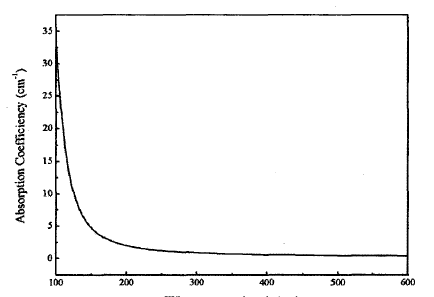
\includegraphics[width=0.62\textwidth]{image/image1.png}
    \bicaption{单图示例}{Single image example}
    \label{fig:single-image-example}
    \fignote{注：如有需要可对图片进行注释说明，标尺内容，英文简称，统计值等，不用可省略。\par 图片来源：如需对图片来源进行说明，请参照此格式，不用可省略。}
\end{figure}

正文文字正文文字正文文字正文文字正文文字正文文字正文文字正文文字正文文字正文文字正文文字正文文字正文文字正文文字正文文字正文文字正文文字正文文字正文文字正文文字正文。

% 如果一个图由两个或两个以上分图组成时，各分图分别以(a)、(b)、(c)……作为图序，
% 并须有分图名，分图名直接列在各自分图的正下方，主图名列在所有分图的下方正中。

\section{标题}
正文文字正文文字正文文字正文文字正文文字正文文字正文文字正文文字正文文字正文文字正文文字正文文字正文文字正文文字正文文字正文文字正文文字正文文字正文文字正文文字正文。

\subsection{标题}
正文文字正文文字正文文字正文文字正文文字正文文字正文文字正文文字正文文字正文

\subsubsection{标题}
\begin{figure}[htbp]
    \centering
    \begin{minipage}[t]{0.48\textwidth}
        \centering
        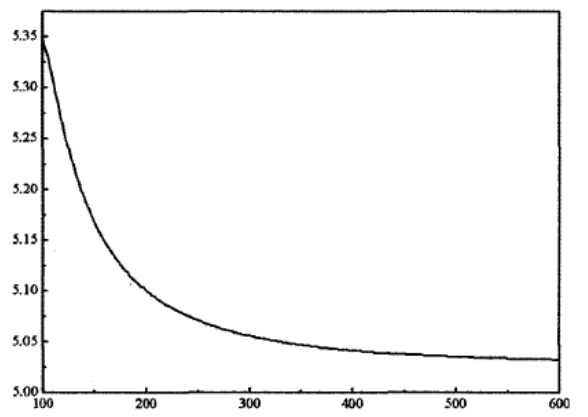
\includegraphics[width=\textwidth]{image/image2(a).png}
        
        {\songti\rmfamily\xiaosi (a)\quad 分图示例一\par}
    \end{minipage}\hfill
    \begin{minipage}[t]{0.48\textwidth}
        \centering
        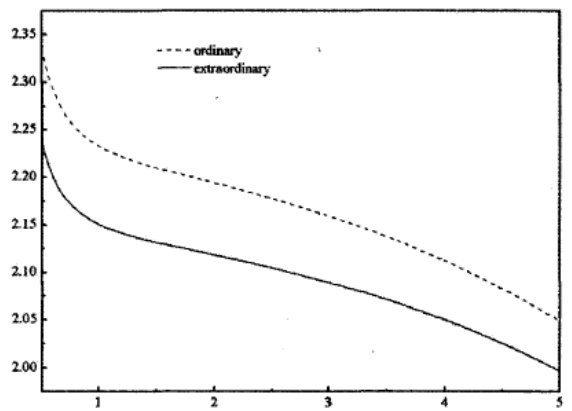
\includegraphics[width=\textwidth]{image/image2(b).png}
        
        {\songti\rmfamily\xiaosi (b)\quad 分图示例二\par}
    \end{minipage}
    \bicaption{双图示例}{Two-image example}
    \label{fig:two-image-example}
\end{figure}

\section{标题}
正文文字正文文字正文文字正文文字正文文字正文文字正文文字正文文字正文文字正文文字正文文字正文文字正文文字正文文字正文文字正文文字正文文字正文文字正文文字正文文字正文。

% 第四章 讨论（每一章必须另页起）
\chapter{讨论}
正文文字正文文字正文文字正文文字正文文字正文文字正文文字正文文字正文文字正文文字正文文字正文文字正文文字正文文字正文文字正文文字正文文字正文文字正文文字正文文字正文文字正文文字正文文字正文文字。

\section{标题}
正文文字正文文字正文文字正文文字正文文字正文文字正文文字正文文字正文文字正文文字正文文字正文文\cite{mayWillLargeComplex1972}字正文文字正文文字正文文字正文文字正文文字正文文字正文文字正文文字正文文字正文文字正文文字正文文字。

\subsection{标题}
正文文字正文文字正文文字正文文字正文文字正文文字正文文字正文文字正文文字正文文字正文文字正文文字正文文字正文文字正文文字正文文字正文文字正文文字正文文字正文文字正文文字正文文字正文文字正文文字。

正文文字正文文字正文文字正文文字正文文字正文文字正文文字正文文字正文文字正文文字正文文字正文文字正文文字正文文字正文文字正文文字正文文字正文文字正文文字正文文字正文文字正文文字正文文字正文文字。

正文文字正文文字正文文字正文文字正文文字正文文字正文文字正文文字正文文字正文文字正文文字正文文字正文文字正文文字\cite{beltranNewTherapiesCastrationresistant2011}正文文字正文文字正文文字正文文字正文文字正文文字正文文字正文文字正文文字正文文字。

% 第五章 总结与展望（每一章必须另页起）
\chapter{总结与展望}
正文文字正文文字正文文字正文文字正文文字正文文字正文文字正文文字正文文字正文文字正文文字正文文字正文文字正文文字正文文字正文文字正文文字正文文字正文文字正文文字正文文字正文文字正文文字正文文字。

正文文字正文文字正文文字正文文字正文文字正文文字正文文字正文文字正文文字正文文字正文文字正文文字正文文字正文文字正文文字正文文字正文文字正文文字正文文字正文文字正文文字正文文字正文文字正文文字。


% ==========================================
% 后置部分 (Back Matter)
% ==========================================
\backmatter

% 致谢 
\chapter{致谢}
正文文字正文文字正文文字正文文字正文文字正文文字正文文字正文文字正文文字正文文字正文文字正文文字正文文字正文文字正文文字正文文字正文文字正文文字正文文字正文文字正文文字正文文字正文文字正文文字。

在正文后对下列各方致谢：

指导完成论文工作的导师、协助导师指导论文工作或提供便利条件的个人或组织（教研室、实验室等）；

在论文工作中提出建议和提供帮助的人；

给予转载和引用权的资料、图片、文献、研究思想和设想的所有者；

其它应感谢的组织和个人。

致谢应实事求是。


% 参考文献 
\printbibliography[title={参考文献}]

% 附录及成果说明
% 附录 
\chapter*{附录 博/硕士在读期间主要研究成果}
\addcontentsline{toc}{chapter}{附录 博/硕士在读期间主要研究成果}

\noindent {\heiti\xiaosan 代表性研究成果}（按时间倒序排序）

\noindent {\heiti\xiaosi 一、期刊论文}

格式: 作者名(本人姓名加粗显示); 论文标题, 期刊名称, 出版年份, 卷(期): 起止页码.

\noindent {\heiti\xiaosi 二、会议论文}

格式: 作者名(本人姓名加粗显示); 论文标题, 会议名称, 会议地址, 起止日期.

\noindent {\heiti\xiaosi 三、专著}

格式: 所有作者（编者姓名）; 专著名称(章节标题), 出版社, 总字数（编者字数）, 出版年份.

\noindent {\heiti\xiaosi 四、授权发明专利}

格式: 发明人（本人姓名加粗显示）; 专利名称, 授权时间, 国别, 专利号.

\noindent {\heiti\xiaosi 五、会议特邀学术报告}

格式: 报告人（本人姓名加粗显示）; 报告名称, 会议名称, 会议地址, 会议时间.

\noindent {\heiti\xiaosi 六、其他成果}

格式: 收录人（本人姓名加粗显示）; 收录案例名称, 发证日期, 发证机构, 证书编号.

\vspace{2em}
\noindent {\heiti\xiaosan 主持或参与科研/临床项目（课题）}（按时间倒序排序）

格式: 资助机构, 项目类别, 名称, 研究起止年月, 获资助金额, 项目状态(已结题或在研等), 主持或参加


\end{document}
